\chapter{SETTING COORDINATE FRAMES}
    \section{Topic}
        \hspace*{0.6cm}Set coordinate frames for the first four links (link 1, link 2, link 3).
    \section{Theory}
    \hspace*{0.6cm}Based on “DENAVIT-HARTENBERG NOTATION” (Lecture 4: Forward Kinematics [1]): Local frame \textbf{$B_i$} to each link (i) at joint $i+1$ is defined as:
    \begin{itemize}
        \item The $z_i$ axis is aligned with the $i + 1$ joint axis.
        \item The $x_i$ axis is defined along the common normal between the $z_i - 1$ and $z_i$
        axes, pointing from the $z_i - 1$ to the $z_i$ axis.
        \item The $y_i$ axis is defined by the right-hand rule.
        \item The origin $o_i$ of the $i$ frame is located at the intersection of the joint axis $i+1$ with the common normal between the $z_i - 1$ and $z_i$ axes.
    \end{itemize}

    \section{Application}
    \begin{figure}[H]
        \centering
        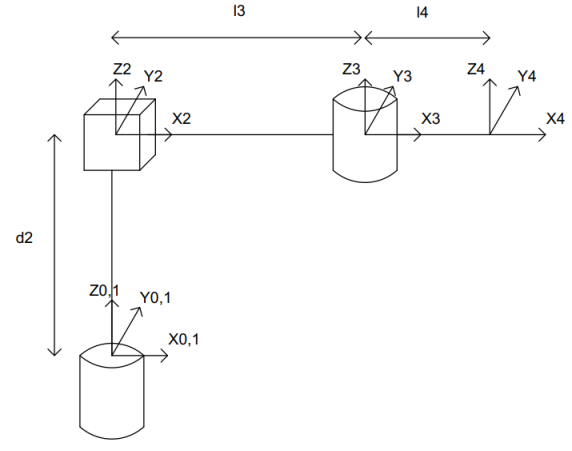
\includegraphics[width=0.7\textwidth]{pictures/set_frame.png} 
        \caption{Setting coordinate frames for robot}
    \end{figure}
